%%%%%%%%%%%%%%%%%%%%%%%%%%%%%%%%%%%%%%%
% Header                              %
%%%%%%%%%%%%%%%%%%%%%%%%%%%%%%%%%%%%%%%
% 
% Revisions: 2017-12-12 Martin Raedel <martin.raedel@dlr.de>
%                       Initial draft
%               
% Contact:   Martin Raedel,  martin.raedel@dlr.de
%            DLR Composite Structures and Adaptive Systems
%          
%                                 __/|__
%                                /_/_/_/  
%            www.dlr.de/fa/en      |/ DLR
% 
%%%%%%%%%%%%%%%%%%%%%%%%%%%%%%%%%%%%%%%
% Content                             %
%%%%%%%%%%%%%%%%%%%%%%%%%%%%%%%%%%%%%%%

\begin{tikzpicture}[
  every node/.style={font=\figurefontsize},
  %inner sep=0pt,
]
  % External figure
  \node[anchor=south west,inner sep=0] (image) at (0,0) {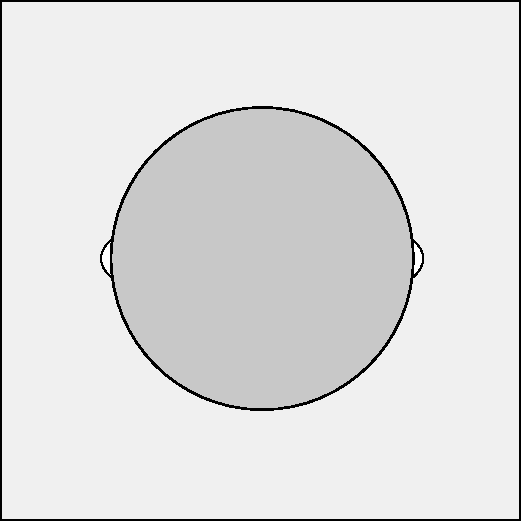
\includegraphics[width=\figwidth]{Obs_Damage_Single_Fiber_I_Crack_Nucleation}};
  % Figure scope
  \begin{scope}[
    x={(image.south east)},
    y={(image.north west)},
  ]
    
    % Load arrows
    \foreach \y in {0,1,...,\numarrows} {\draw[-latex] (-0.025,\y/\numarrows) -- (-0.15,\y/\numarrows) coordinate (loadarrowleft\y);}
    \foreach \y in {0,1,...,\numarrows} {\draw[-latex] ( 1.025,\y/\numarrows) -- ( 1.15,\y/\numarrows) coordinate (loadarrowright\y);}
    
    % Labels
    %\node[anchor=south west,inner sep=1pt] (matrixlabel) at (0.015,0.015) %{Matrix};
    %\node[anchor=north east,inner sep=1pt] (fibrelabel)  at (0.985,0.985) {Fibre};
    %\draw[thin] (fibrelabel) -- (0.6,0.6);
    
    % Help grid and labels
    %\draw[help lines,xstep=.1,ystep=.1] (0,0) grid (1,1);
    %\foreach \x in {0,1,...,9} {\node [anchor=north] at (\x/10,0) {0.\x};}
    %\foreach \y in {0,1,...,9} {\node [anchor=east]  at (0,\y/10) {0.\y};}
  \end{scope}
\end{tikzpicture}